\documentclass[12pt,a4paper,twoside]{article}

\usepackage{fancyhdr}
\usepackage{lastpage}
\usepackage{a4wide} 
\usepackage{amsmath}
\usepackage{amssymb} 
\usepackage{graphicx}
\usepackage{color}
\usepackage{fancybox}
\usepackage{moreverb}
\usepackage{listings}
\usepackage[utf8]{inputenc}
\usepackage[T1]{fontenc}
\usepackage[toc,page]{appendix}
\usepackage{hyperref}
\usepackage{subcaption}
\usepackage{booktabs}

%\fbox{}
%\shadowbox{}
%\doublebox{}
%\ovalbox{}
%\Ovalbox{}
%\shabox{}


% --- Logo ---
%\makebox[\textwidth][l]{
%\raisebox{-15pt}[0pt][0pt]{
%\hspace{2.5cm}
%\includegraphics[scale=0.1]{Images/logo_atos.eps}
%}
%}
\title{Final year project report}
\author{Adrien Gregorj}
\date{\today}

\pagestyle{headings}

\begin{document}
\lstset{ numbers=left, tabsize=3, frame=single, numberstyle=\ttfamily, basicstyle=\footnotesize} 
\thispagestyle{empty}

\begin{center}
\makebox[\textwidth][l]{
\raisebox{-8pt}[0pt][0pt]{

\includegraphics[scale=0.06]{images/OU_banner}
}
}
\makebox[\textwidth][r]{
\raisebox{0pt}[0pt][0pt]{
\includegraphics[scale=0.2]{images/logo_ensimag}
}
}
Grenoble INP  -- Ensimag\\
École Nationale Supérieure d'Informatique et de Mathématiques Appliquées\\
\vspace{3cm}
{\LARGE Final year project pre-report}\\
\vspace{1cm}
Performed at Okayama University\\
\vspace{2cm}
\shadowbox{
\begin{minipage}{1\textwidth}
\begin{center}
{\Huge Human behavior analysis}\\
\end{center}
\end{minipage}
}\\
\vspace{3cm}
Adrien Gregorj\\
3$^{\text{rd}}$ year -- Option MMIS Bio\\
\vspace{3mm}
19$^{\text{th}}$ February, 2018 -- 20$^{\text{th}}$ July, 2018\\
\vspace{4cm}
\begin{tabular}{p{10cm}p{10cm}}
{\bf Okayama University}                                     & ~~~~~~~~~~~~~~~~~~~~{\bf Supervisor}\\
{\footnotesize 1-1, Tsushima-Naka, 1-Chome}                           & ~~~~~~~~~~~~~~~~~Akito Monden\\
{\footnotesize Okayama 700-8530}                                        & ~~~~~~~~~~~~~~~~~{\bf School Tutor}\\
{\footnotesize Japan}                         & ~~~~~~~~~~~~~~~~~James Crowley\\
\end{tabular}
\end{center}
\newpage

\tableofcontents

\newpage

\section{Context}

\subsection{Home structure}
This internship takes places in an academic context. The home structure is the Graduate School of Natural Science and Technology of Okayama University. In particular the host laboratory is part of the Division of Industrial Innovation Sciences, in the Department of Computer Science.

Okayama University is a well ranked university in Japan located in Okayama Prefecture, in the Chugoku region (westernmost region) of the main island of Honshu. The school was founded in 1870 and welcomes around 14000 students (10000 undergraduates, 3000 postgraduates and 1000 doctoral students). It's motto is \guillemotleft~Creating and fostering higher knowledge and wisdom \guillemotright.

The Graduate School of Natural Science and Technology was originally established in April 1987. It focuses on research in the fundamental sciences such as global climate change, plant photosynthesis or supernova neutrinos and the Division of Industrial Innovation Sciences especially works on applied engineering in the field of computer science, robotic, material sciences and more. 

In the Department of Computer Science, the topics of research are the basic theory and application of information technology, artificial intelligence and computer technology. Examples of research projects includes the development of a visualization tool for a processor or human tracking algorithm by means of attention control. Dr Akito Monden is the professor of the Theory of Programming and Artificial Intelligence laboratory where this internship takes place and Dr Zeynep Yücel is the assistant professor in the same laboratory. 

\section{Problematic}

\subsection{State of the existing}
Dr Zeynep Yücel has been working for a few years on modeling crowd movements~\cite{Zanlungo2017}\cite{Yucel2013}\cite{Yucel2017}. The motivation behind constructing such models are numerous: testing architectural designs for an evacuation process, designing accurate crowd models for movies or video games, etc. Japan being very involved in the robotic industries, these projects guidance was to analyse comportements of pairs of pedestrian (we will refer such a group as a dyad in the rest of this report) to potentially develop robots able to walk along side with people in the most natural manner. In order to get real data that could be analysed and from which mathematical models could be derived, cameras and sensors were installed in an underground pedestrian zone. 

Previous work (\cite{Yucel2013}) has also shown that using trajectory informations, the composition of a group can be accurately determined. Detection of dyads can be performed relying on data from the sensors that represents the trajectories of the pedestrians.

\subsection{Objectives}
One of the main challenge behind pedestrian modelling is to take into account the interaction between them. Indeed,~\cite{Yucel2017} as demonstrated that the motion patterns of individual performing gestures (i.e.~touching each others, looking at each other, looking at a common target or speaking together) are significantly different from the ones of not interacting individuals. The data used for this work relied on human annotations of the videos to evaluate the presence or absence of gestures.

The goal of this project is to develop a pipeline to automatize the classification process of the dyads gestures. Instead of relying on human referees to decide wether or not a couple of pedestrians are interacting in a given video, this decision should be made by an algorithm. Indeed, the annotation process is long and tedious and mistakes are often introduced as annotators might spend several hours doing this repetitive and unexciting task.

Given a set of input data (video files and trajectory, this will be described more precisely in~\ref{sec:input}), the algorithm needs to extract portions containing groups of two pedestrians and perform a treatment of the video portion to decide if they are interacting.

It is important to note that the algorithm might rely on previous annotations made by coders if supervised machine learning methods are used. Yet it should be able to generalize the classification process to new videos given that they are similar to the one already captured in terms of point of view. Difference of lighting and exposition should be handled.

Two primary milestones can be set in this project.

The first step consists in being able to partition interacting dyads from non-interacting dyads, without any distinction among the kind of gestures that is being performed. The expected results for this task should be greater than 80\% accuracy (more than 80\% of the dyads should be rightly classified).

Later on, we wish to be able to classify more precisely the action performed. For this more complex task, an accuracy greater than 70\% should be achieved. 


\section{Proposed solution}

The current pipeline that we wish to implement is as described in this section. Figure~\ref{fig:pipeline} describes the main steps involved. Globally, the first steps consists of video preprocessing to extract the part of the raw videos that involves dyads passing by and to conserve only the parts where gesture detection makes sense (pedestrian walking too far away from the camera are too small to be analysed accurately). This step should provide one short video clip for each dyad. Then pose estimation of the pedestrian can be performed on those preprocessed video clips to extract two skeletons for each frame. Finally, these skeletons can be used as input in Graph Neural Network to perform action classification for the dyads. This section will present in details these steps and the encountered challenges.  

\begin{figure}
    \centering
        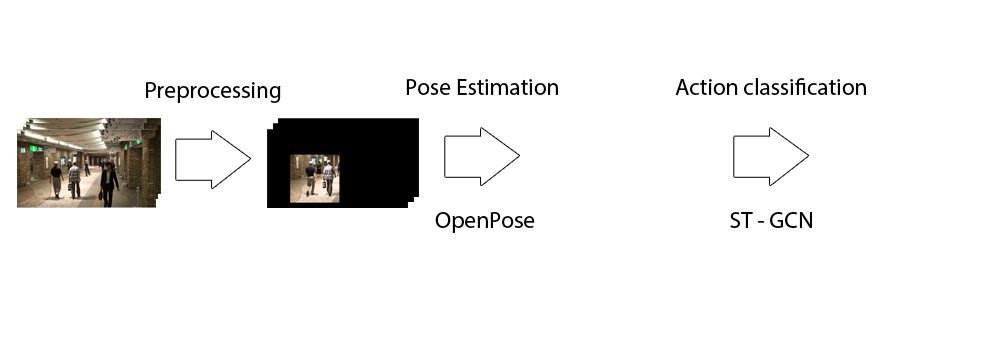
\includegraphics[width=0.8\textwidth]{images/pipeline}
    \caption{Schema of the pipeline of the project.}
    \label{fig:pipeline}
\end{figure}

\subsection{Input data}
\label{sec:input}

This section describes the initial data that is used along the pipeline. 

\begin{description}
    \item[video files:] set of 15 minutes successive video files (\texttt{MTS} format). The camera was set in a underground pedestrian pathway (see figure~\ref{fig:preprocessing} for an example).
    \item[trajectories:] set of trajectory data file. There is one file for each pedestrian. They were obtained using Laser Range sensors that scanned the pathway to get horizontal data points located approximately around the torso of the pedestrians. Each file consists of a list of x and y coordinates associated with Unix timestamps that corresponds to the date and time for the position. For each file, its name corresponds to the ID of the pedestrian. This ID are the same as the one used in the annotation file.
    \item[annotations:] one csv file that indicates for each pedestrian (using its ID) the interaction it is involved in. This includes the number of person the pedestrian is interacting with (ranging from 0 to 7). The kind of gesture he is performing (none, gazing at someone, touching someone, speaking with someone or gazing at a common target). This annotations were established by human coders and therefore contains potential errors.
\end{description}

\subsection{Pre-processing}
The raw videos from the camera need to be modified in order to be treated. Indeed, the relevant portions that can later be processed by the neural networks need to be selected. 

The first step is to retrieve all the dyads contained in the videos. This is done by using the annotations files and listing all the pedestrian that interacts with one and only one other pedestrian (we do not consider groups larger than two). We can then retrieve the corresponding trajectories using the IDs of the two members of the dyad.

As the trajectory are defined with Unix timestamps, with absolute values, calibration needs to be perform to find the related time in the video that corresponds to a given point. In the first video, the time of the Laser range sensor (which is the one of the trajectory) is shown on a computer screen, which allows to find a reference point. As all videos are directly following one another, but are not exactly the same time, I wrote a script to save the duration of all videos along with their name in a file. This file can be used to find the videos in which a trajectory is actually visible by summing all the duration of the first videos until it is larger than the beginning of the trajectory, thus giving the name of the video in which it appears. The time trajectory can then be expressed relatively to the beginning of the video. 

I choose to consider the trajectory of the middle point between the two pedestrians, that can then be used to compute a bounding box that contains both pedestrians. The trajectory of the two people in a dyad do not necessarily starts at the same time as they do not enter the range of the sensors at the same time. Thus, the biggest matching time portion between the two trajectory had to be computed. Then for each two points in this time portion, the middle point was computed (see figure~\ref{fig:trajectories}).

\begin{figure}
    \centering
    \begin{subfigure}[b]{0.45\textwidth}
        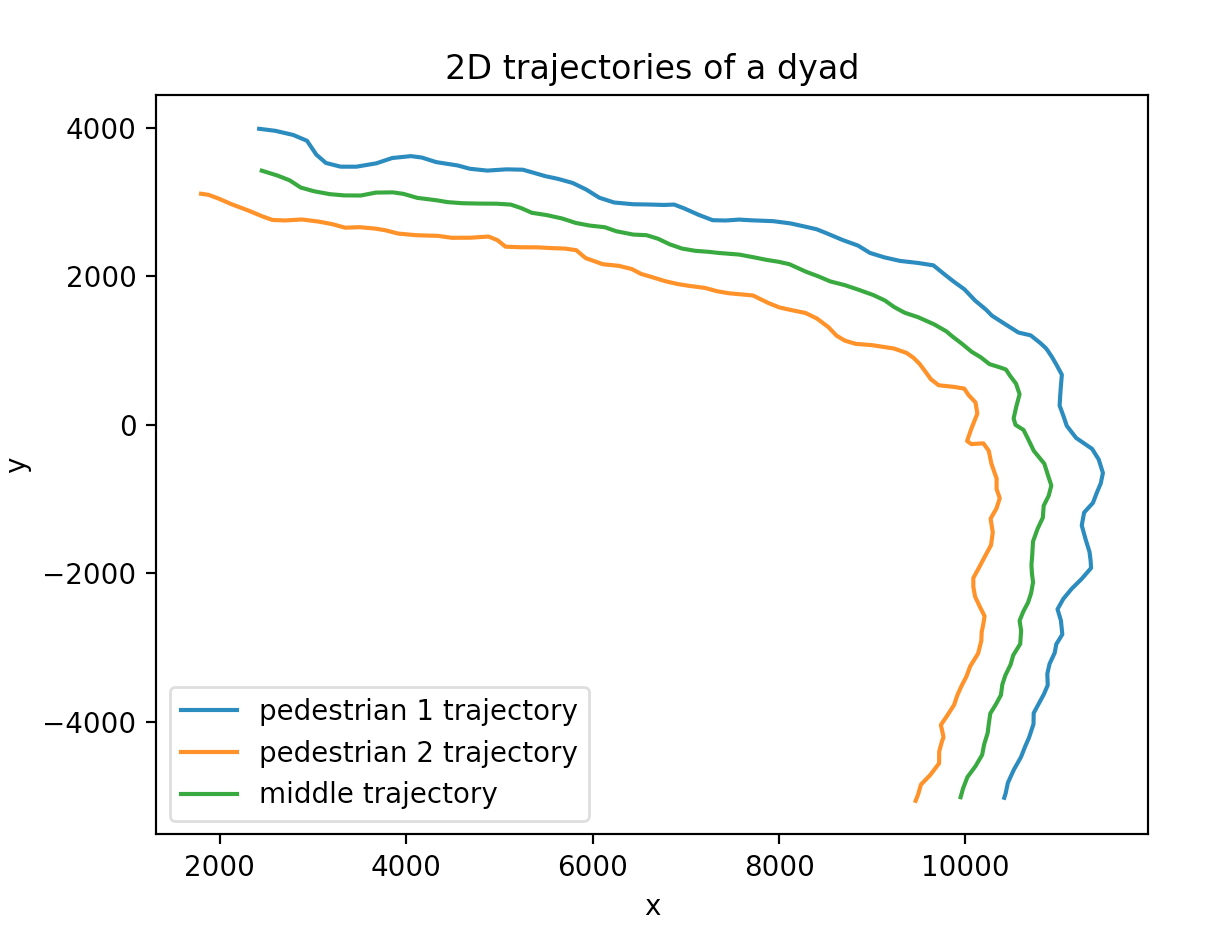
\includegraphics[width=\textwidth]{images/traj1}
    \end{subfigure}
    ~
    \begin{subfigure}[b]{0.45\textwidth}
        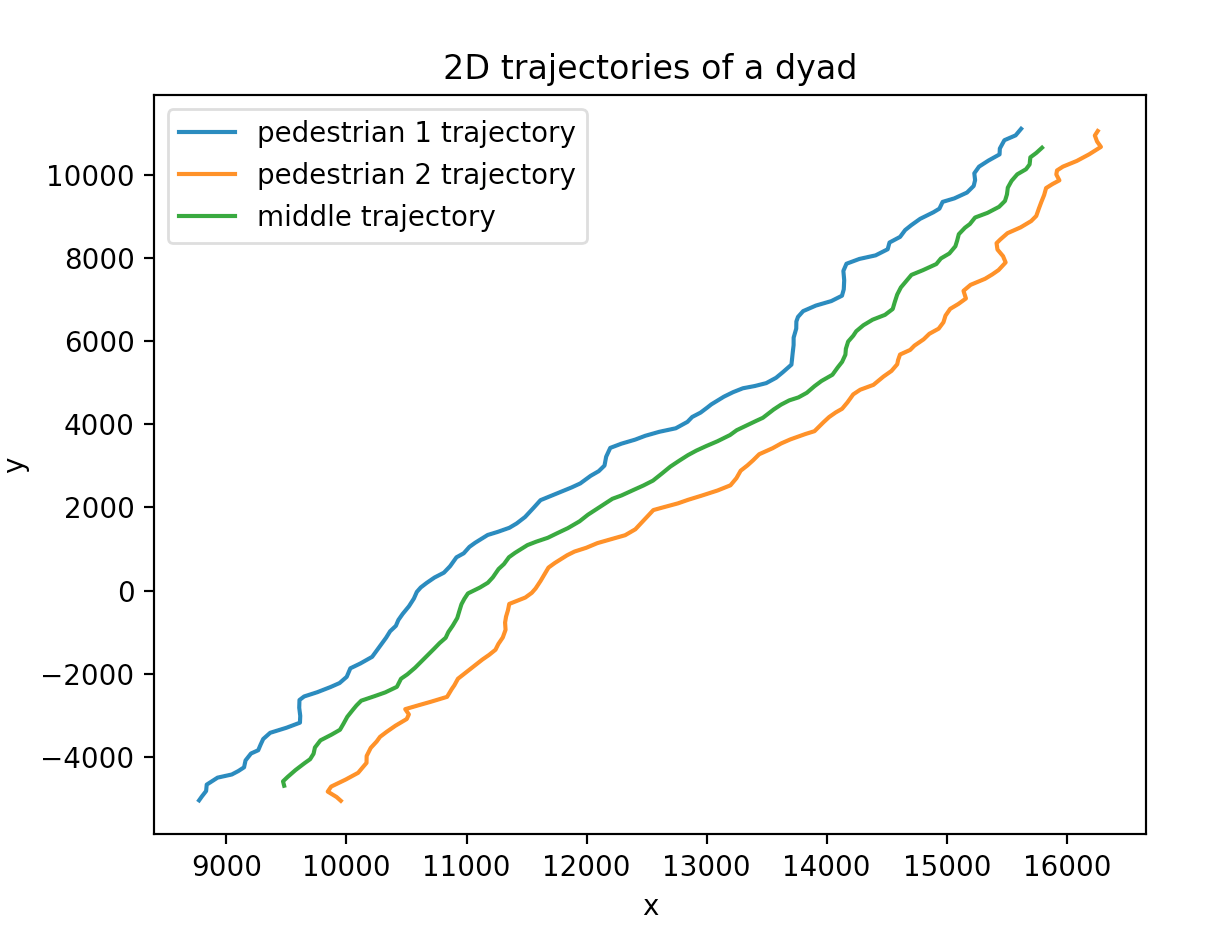
\includegraphics[width=\textwidth]{images/traj2}
    \end{subfigure}
    \caption{Plot of some dyads trajectory in the horizontal 2D plan.}
    \label{fig:trajectories}
\end{figure}


In order to be able to map the trajectories to the video to find the appropriate portion to extract, the camera calibration matrix needs to be computed. This is done using OpenCV calibration tool box. In the considered case, no calibration rigs were used but the world coordinates of the sensor poles that appears in the images were known and their coordinates in the image referential could be computed. As there is a height difference in the corridor, the sensor closer to the camera are not on the same plan than the furthest one. The OpenCV toolbox does not provide a calibration function that can compute the camera matrix using a set of non planar points (a set of 3D coordinates in the world referential and their 2D matchs in the image referential) unless an input guess is given. For this initial guess I used values previously used for similar works, and the results were satisfying (see figure~\ref{fig:calibration}).

\begin{figure}
    \centering
        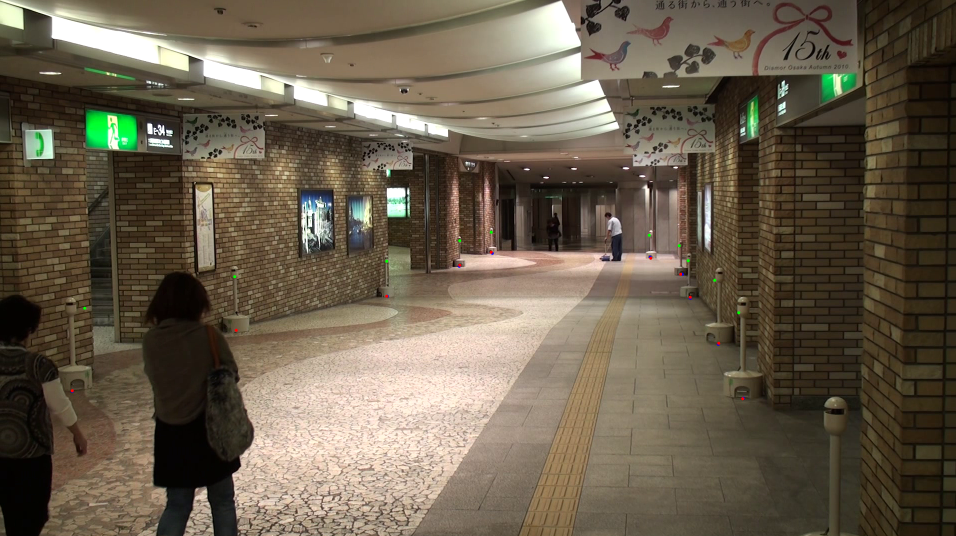
\includegraphics[width=0.8\textwidth]{images/calibration}
    \caption{Illustration of the calibration results, red dots corresponds to the 2D points used in the image referential, blue dots to the 2D mapping of the 3D points located at the bottom of the pole (that should corresponds to the red dots) and green dots to the 2D mapping of the 3D points located at the top of the sensors (the height of the points is the height of the bottom points plus 85 centimeters). }
    \label{fig:calibration}
\end{figure}

The sensor only provides 2D coordinates corresponding to a point 40 cm high at the center of the torso of the pedestrian. The $z$ value was then computed by approximating the actual topology of the corridor. A rough estimation can be made to compute the height difference due to the slope in the middle. This estimation can thereafter be used to compute the height of the foot of the pedestrian for example and plot a dot using OpenCV to validate the trajectory mapping (see figure~\ref{fig:middle_point_traj}).


\begin{figure}
    \centering
    \begin{subfigure}[b]{0.45\textwidth}
        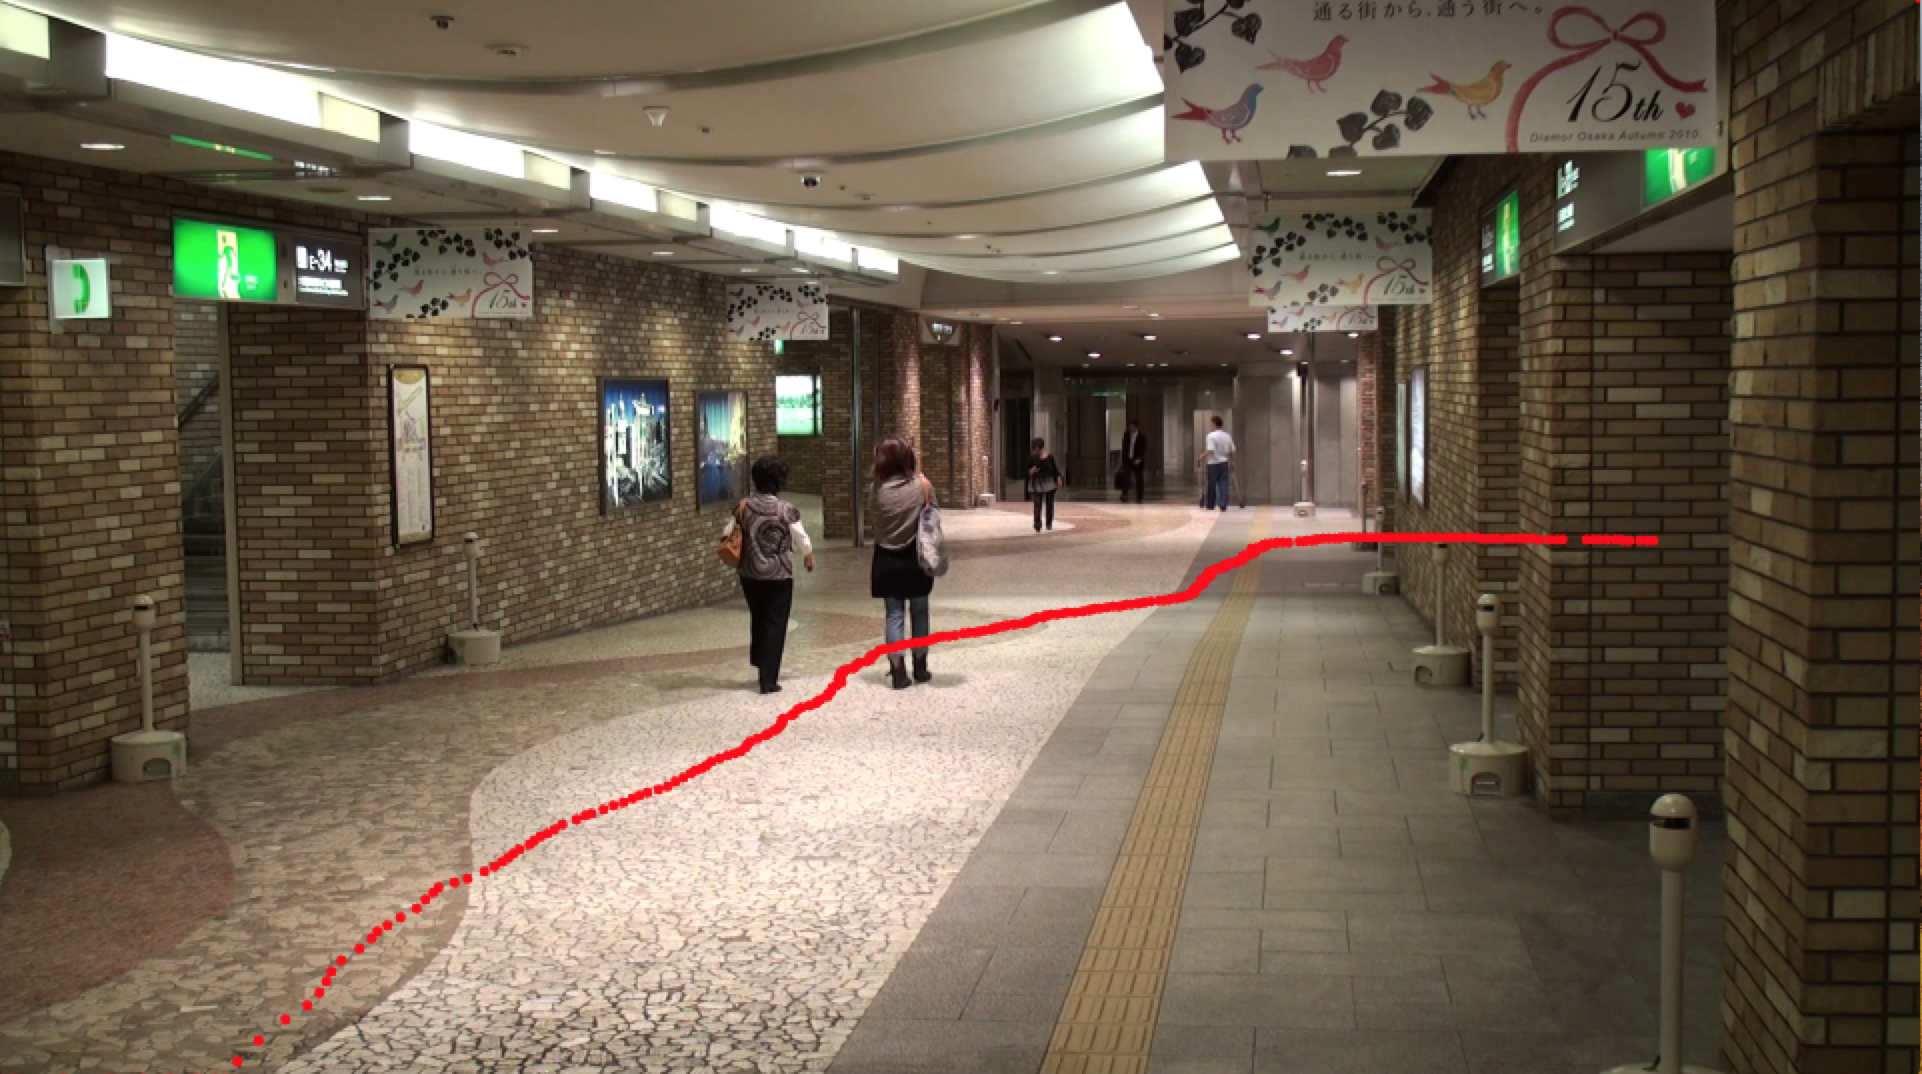
\includegraphics[width=\textwidth]{images/middle_point_traj}
        \caption{}
        \label{fig:middle_point_traj}
    \end{subfigure}
    ~
    \begin{subfigure}[b]{0.45\textwidth}
        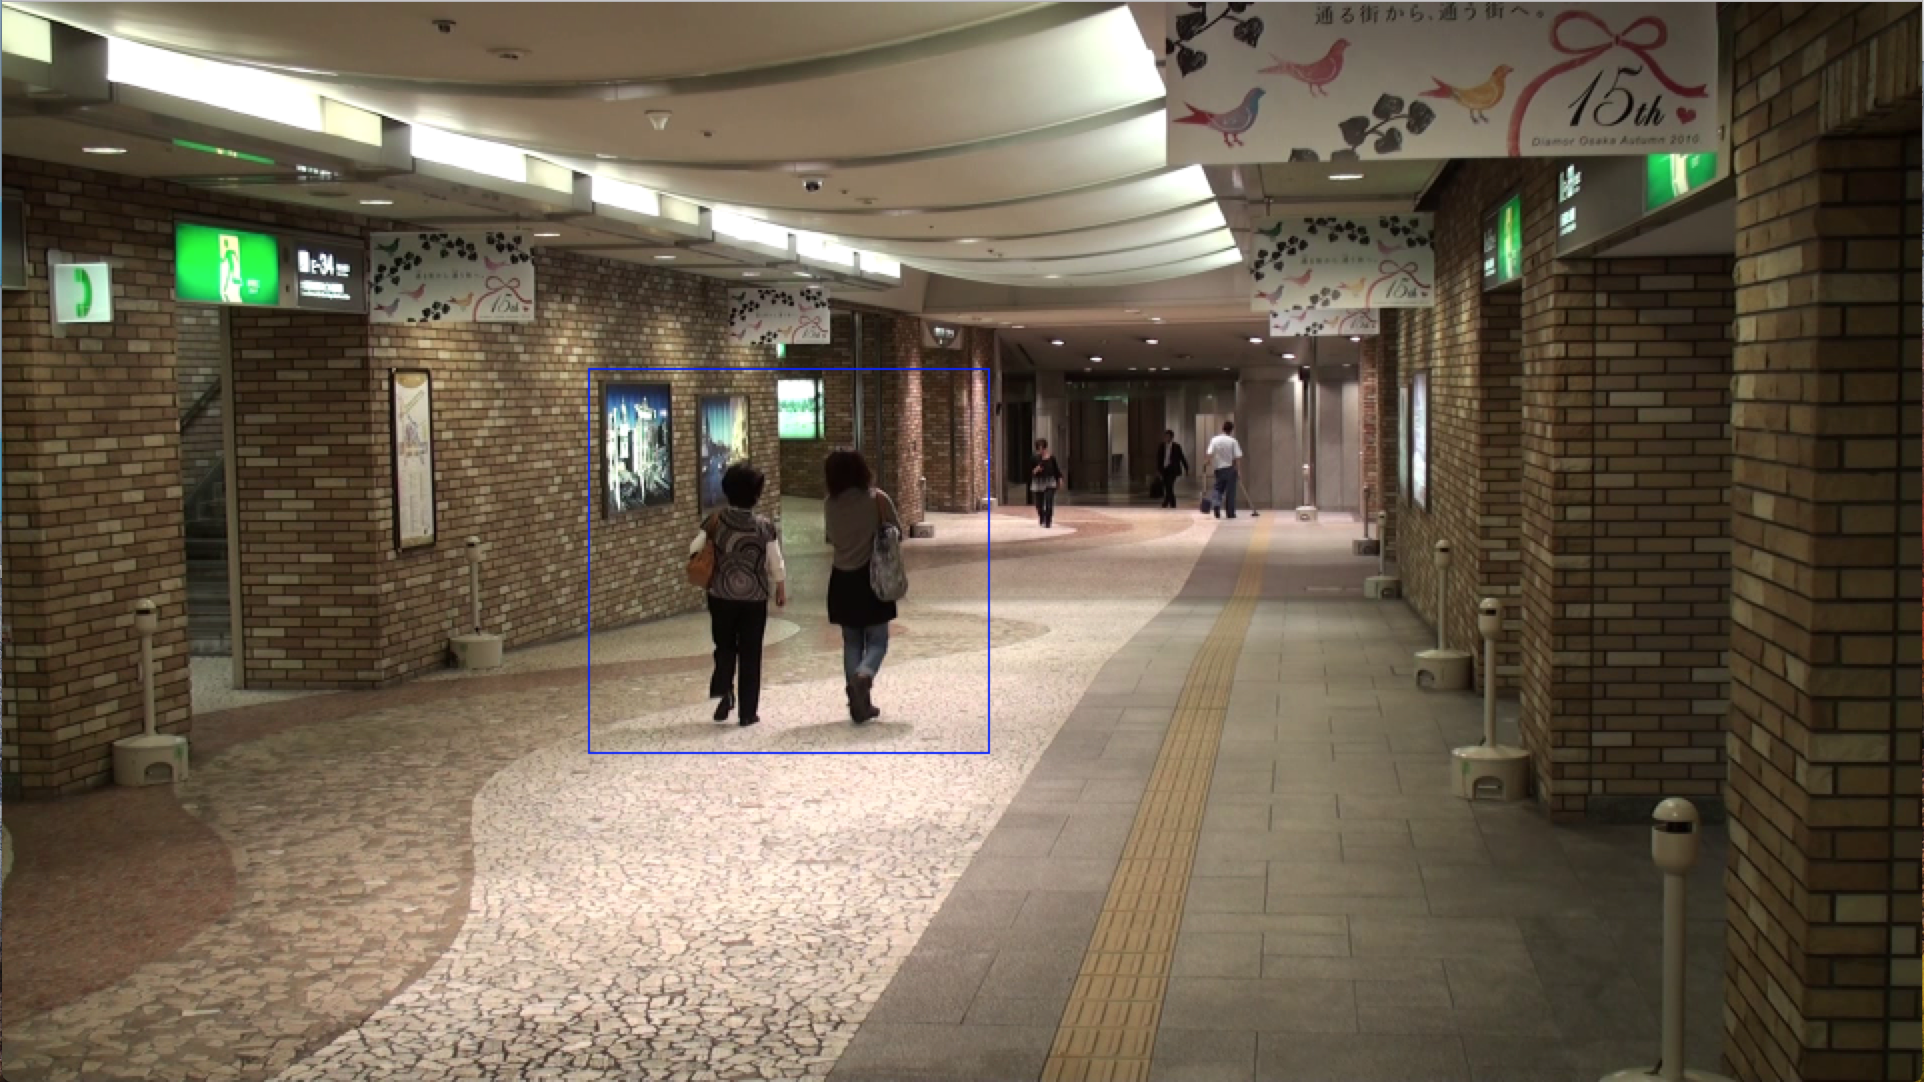
\includegraphics[width=\textwidth]{images/bounding_box}
        \caption{}
        \label{fig:bounding_box}
    \end{subfigure}
    ~
    \begin{subfigure}[b]{0.45\textwidth}
        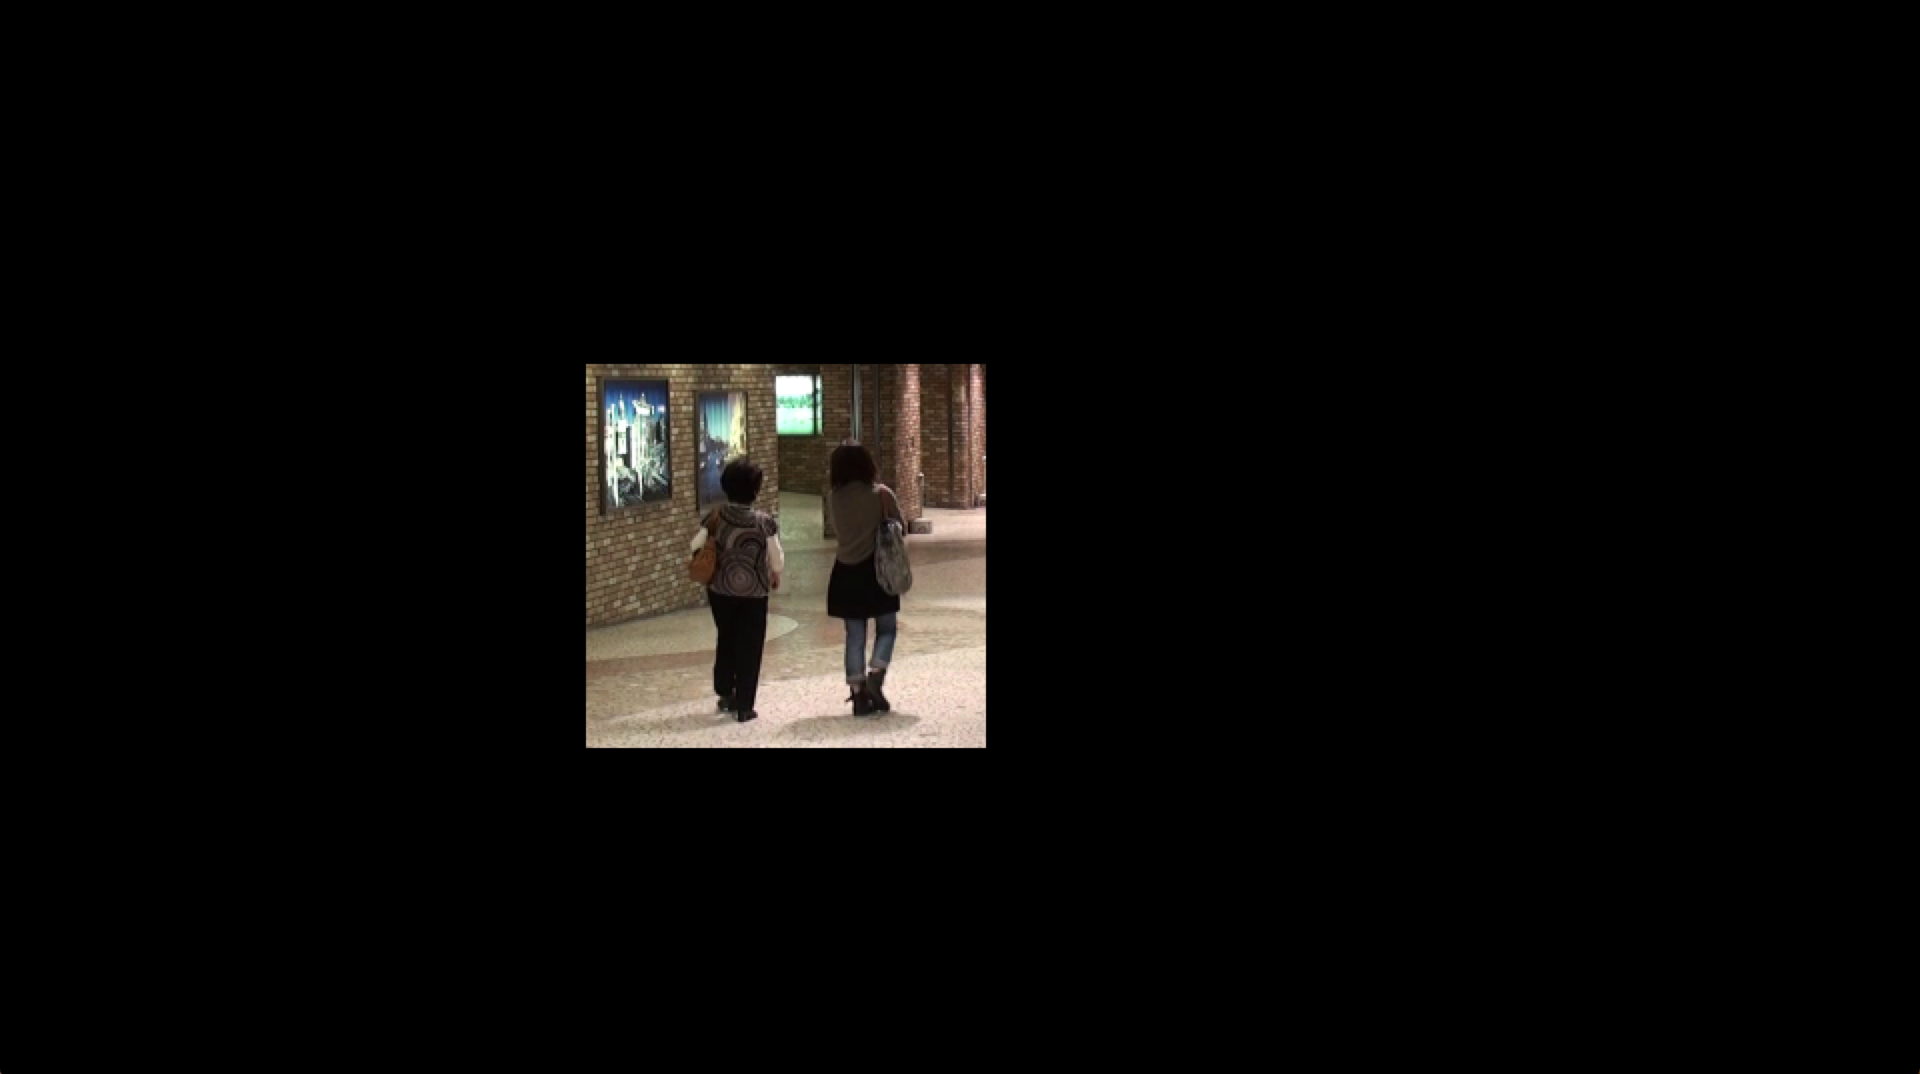
\includegraphics[width=\textwidth]{images/masked}
        \caption{}
        \label{fig:masked}
    \end{subfigure}
    \caption{Illustration of the various steps of the preprocessing.~\ref{fig:middle_point_traj} shows the middle point mapped back to the video,~\ref{fig:bounding_box} shows the computed bounding box and~\ref{fig:masked} the results of the subtraction using the bounding box as a mask.}\label{fig:preprocessing}
\end{figure}

The trajectory of one given dyad is generally not entirely interesting. Indeed most of it (and sometimes all of it) takes place too far away from the camera to be able to properly to a pose estimation (see the next subsection); and sometimes the pedestrian are also too close and partially out of frame. Thus a spatial \guillemotleft~portion of interest \guillemotright~was defined and only the portion of the video that corresponds to the pedestrians walking in this portion was kept.

To compute the actual portion of the screen that contains the walking dyad, a bounding box has been mapped from the real world to the image plan, using the camera matrix computed with the calibration. In the world coordinates, the bounding box is 3 meters wide and 2 meters high so that it surround the two pedestrian. The middle of the bounding box corresponds to the middle point trajectory computed previously. This bounding box is then used as a mask using the OpenCV toolbox to subtract all the unnecessary information (see figures~\ref{fig:bounding_box} and~\ref{fig:masked}).

\subsection{Pose estimation}
The pose estimation process is run using the OpenPose library which is publicly available. The algorithm used is based on body parts inference to identify joints in every frame~\cite{Cao2016}. This project is currently state of the art for the pose estimation problem. This section will briefly explain the algorithm operation.

The model is mainly composed of a multi-stage Convolutional Neural Network that evaluates the confidence maps for body parts (18 different joint: right and left elbow, right and left feet, etc.) but also what the authors of the paper call \guillemotleft~part affinity fields \guillemotright~(PAF) which correspond to vectors that encode the direction between the two joints for each pixel on a given limb. Multiple passes allows to iteratively raffine the detection to avoid false detection (right wrist instead of the left one for example). 

A graph can be modeled using the detected body parts as vertices and by scoring the edges using the part affinity fields with the outputs provided by the neural network. The integral of the PAF over the line that join the two parts gives a cost that encode the confidence In order to retrieve actual skeletons from this graph, which is an NP Hard problem, the authors  introduced a greedy algorithm that perform well and rapidly. They actually subdivided the problem to work on smaller bi-partite graphs (considering successively all the joints association: right wrist - right elbow, right foot - right knee, etc.) instead of considering all the joints at once.

The toolbox performs well on the preprocessed videos even for the pedestrian walking away from the camera (see~\ref{fig:skeleton}) for whom detecting facial keypoints (nose, eyes and mouth) is impossible. Moreover it comes with a wide diversity of parameters that allows to store extracted skeletons for examples, as detailed in the following section.

\begin{figure}
    \centering
        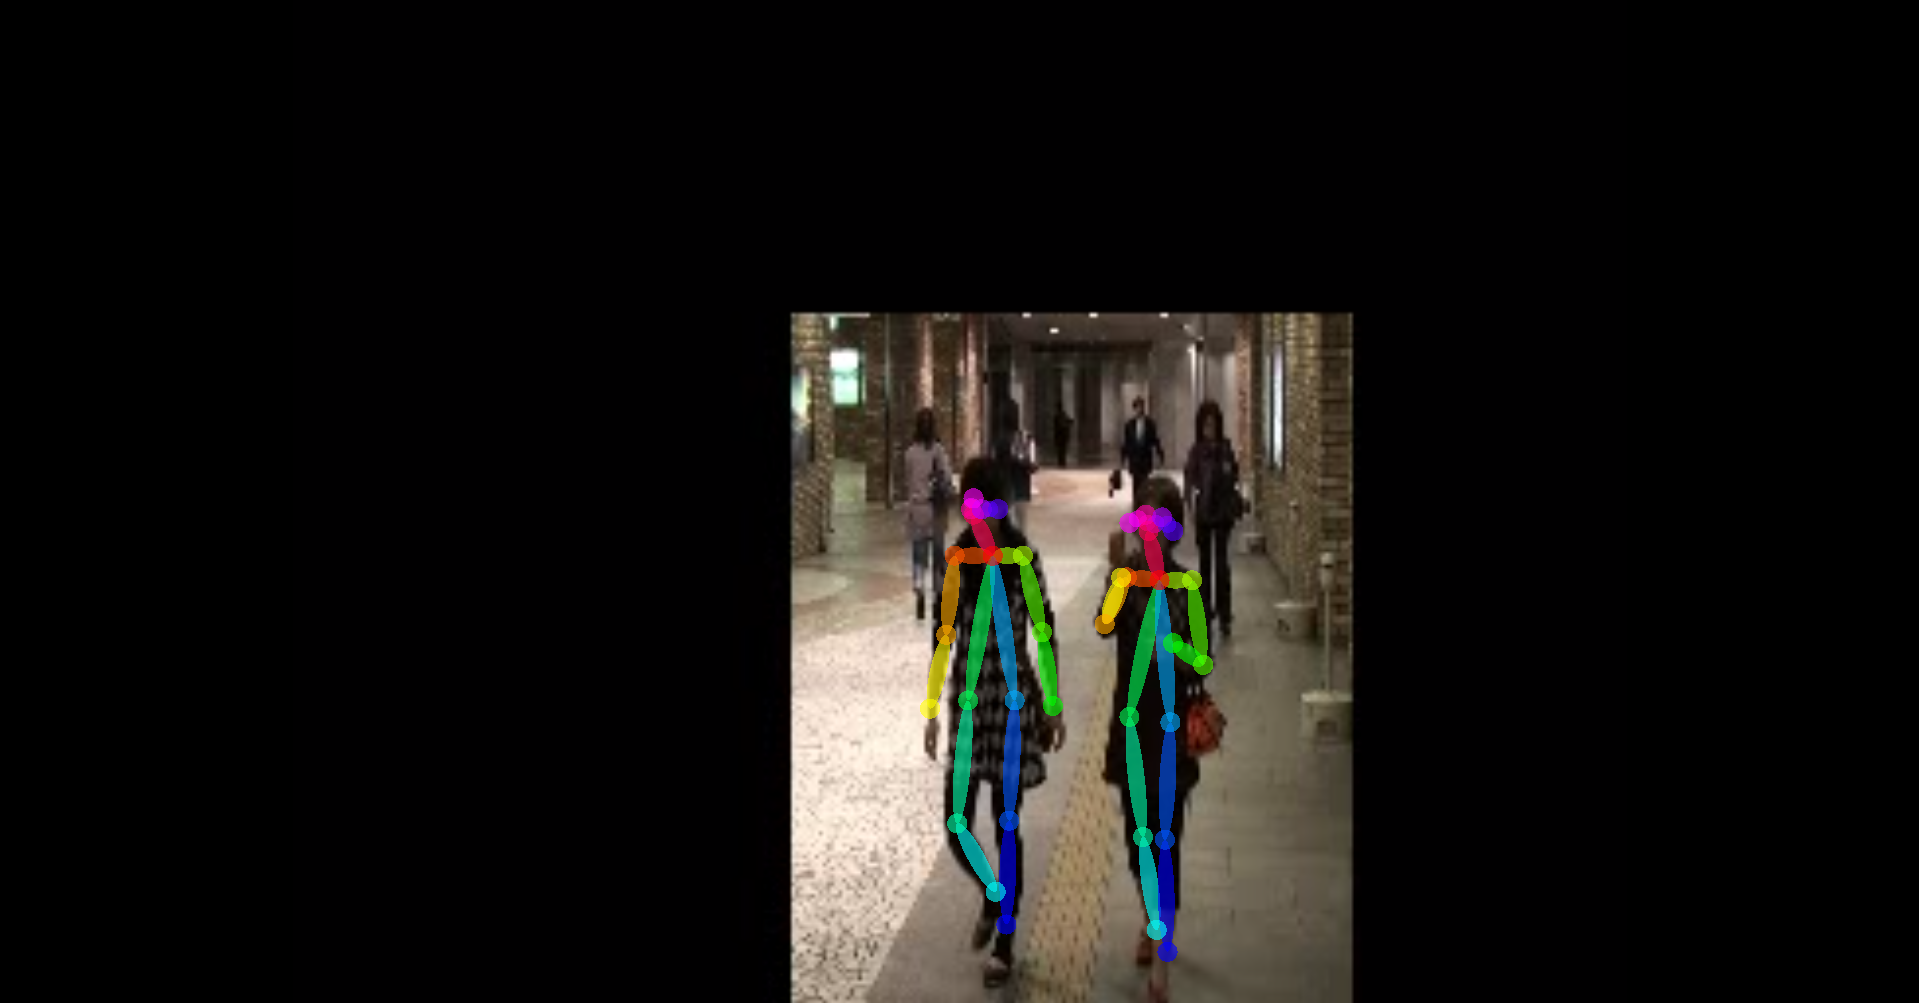
\includegraphics[width=0.7\textwidth]{images/dyad_rendered}
    \caption{Examples of skeleton pose estimation on a preprocessed videos. The number of detection was limited to two detections (keeping the ones with the best average confidence score.)}
    \label{fig:skeleton}
\end{figure}

\subsection{Action classification}
I plan on using machine learning algorithms to classify the video clips. For a start, the classifier should be able to distinguish dyads performing any kind of gestures from dyads not doing anything else than walking. Later the goal will be to be able to get 5 classes corresponding to the 4 gestures and 1 class for the absence of gesture.

A bibliography study pointed me toward~\cite{Yan2018} which describes a Graph Convolutional Network to perform action recognition on skeleton pose flows and that proposes publicly available source code on GitHub. The st-gcn repository provides an neural network trained to classify multiple action classes. This section will briefly explain the key concepts of Graph Convolutional Network (GCN) and the specific characteristics of the Spatio-Temporal GCN introduced in~\cite{Yan2018}.

The idea behind Graph Convolutional Network is that many datasets are actually ordered as graphs or networks and that classical neural networks do not provide efficient and well designed way to treat this kind of data. Recent works have introduced models that can deal with graphs. The input of the network is the adjacency matrix of the graph and a convolution operator can be defined as the inner product between a weight function and the input values of particularly sampled nodes. In a classical image convolution, the sampling function gives the squared neighborhood at a given point. In the graph convolution, the set of neighbors up to a certain distance (distance 1 neighbors being one link away from the node, distance 2, two links away, etc.) of a node can be taken. The weight function is generally defined by labeling the neighbors and assigning weights to labels.
 
In the ST-GCN paper, the graph used can be directly obtained from the inference of the OpenPose algorithm. The spatio-temporal graph is obtained by \guillemotleft~stacking \guillemotright~together the graph obtained at each frame. That means that each node (that corresponds to a specific joint) is linked to itself in the next and previous frame (see figure~\ref{fig:stgcn_graph}).

\begin{figure}
    \centering
        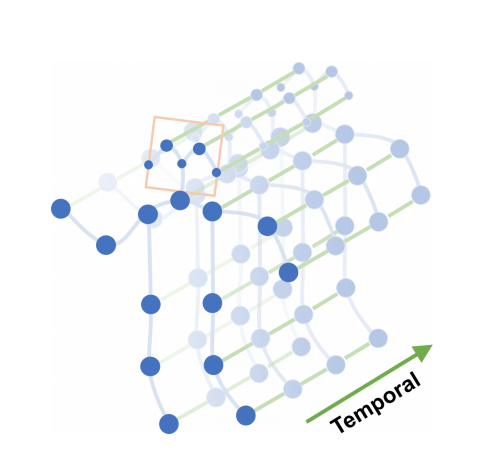
\includegraphics[width=0.5\textwidth]{images/stgcn_graph}
    \caption{Illustration of the ST-GCN graph, from the original paper.}
\label{fig:stgcn_graph}
\end{figure}

A spatial convolution is first defined in this project. The sampling function used is the first order distance and divers labeling methods have been examined by the authors to construct the weights function. The one that achieves the best performance is the \guillemotleft~Spatial Configuration \guillemotright. For this partition, the center of gravity of the skeleton is evaluated. Then the distance from the neighbor nodes of the kernel root node to the center of gravity is computed. In the case where this distance is shorter than the distance between the root node and the center of gravity (centripetal nodes), one label is given, and if this distance is longer (centrifugal nodes), another one is given (see figure~\ref{fig:partition_strat}), resulting in a bipartition of the neighborhood.

\begin{figure}
    \centering
        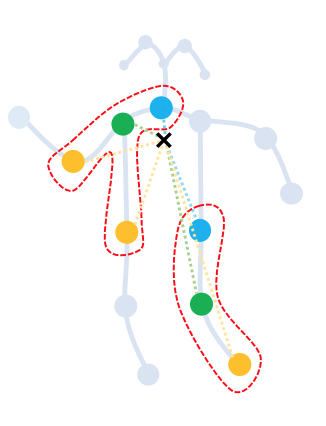
\includegraphics[width=0.2\textwidth]{images/partition_strat}
    \caption{Illustration of the Spatial Configuration partition, from the original paper.}
\label{fig:partition_strat}
\end{figure}

The spatial element is added by also taking neighbors in the spatial direction up to a certain time and labeling them according to the time \guillemotleft~distance \guillemotright~to the frame of the considered node.

The authors provide pretrained model on their github repository. It was trained on Google's Kinetic dataset that contains around 300,000 video clips covering 400 human action classes. They began by using OpenPose algorithm to extract skeletons from all the raw Youtube video clips that compose the dataset. To do so, they first resized the clips to $340 \times 256$ and $30$ FPS. Then, using the OpenPose toolbox, they extracted two times 18 joints for each frame, represented by $(X,Y,C)$ tuples where $X$ and $Y$ are the 2D coordinates of the joint in the frame and $C$ is the confidence score for the joint. The 36 joints correspond to the two people with maximum average confidence score. Every clip is padded by looping over the sequence to produce 300 frames. This process creates a $(3, 300, 18, 2)$ tensor for each video that serves as input to the neural network. 

OpenPose provides an option to write inferred skeleton to JSON files. This creates one JSON file per frame of the input video containing the coordinates and score of all the detected joints, grouped for each detected person. The toolbox also provides options to limit the number of detected people (keeping only the ones with the biggest average confidence) and to normalize the $(X,Y)$ coordinates between 0 and 1 that is very useful to get normalized data for the network.

The OpenPose output format is different than the one used by ST-GCN where one JSON file correspond to one video clip with all the skeleton detected in each frame begin concatenated in one array. I thus created a Python script to convert OpenPose format into ST-GCN format and was able to test the pretrained model on the skeleton data extracted from the preprocessed videos.

As anticipated, the classification obtained is not satisfactory. Indeed, firstly, the Kinetic dataset classes (that are listed at the end of the paper~\cite{Kay2017}) do not fit for this particular classification process. The classes are covering a large set of human actions but do not distinguish different actions performed while walking for example. Moreover, the preprocessed video clips contains big depth variation as the pedestrian are walking toward the camera or away from it. By looking at the way the graph is used in the ST-GCN, we can imagine that it performs better with people acting at a fix distance from the camera and thus keeping a similar size in the video 2D plan. 

For those reason, the nex step will be to try and train a model on the pedestrian video clips using the annotations as ground truth. According to the performance that can be achieved using this newly trained model, it will probably be necessary to adapt the model or the data to compensate the depth change. I plan on trying to normalize the extracted skeleton according to the size of the bounding box. Indeed, this should ensure that size of the skeleton are consistent between the frames.

Another issue that I am experiencing is that sometimes another pedestrian (not part of the dyad) appears in the video and can obstruct the dyad or just get better confidence score and thus provide a bad skeleton instead of the one that should be provided by members of the dyad. I plan on performing some consistence check to only keep skeleton that can belong to the same person from one frame to another. Computing average distance between the joints of the skeleton in two frames and only keeping the one with the lowest distance could suffice to provide time consistent skeletons, given that the first one taken in account is actually from a pedestrian in the dyad. 

\subsection{Evaluation}
Using the ground truth provided by human referees, diverse evaluation procedure can be derived based on error measures for this classification problem. Popular metrics to evaluate the performance of a classification system exist, such as precision and recall  or plotting receiver operator characteristics curves. The accuracy of the classifier can also represents a simple evaluation metric.

The usual procedure used to evaluate supervised machine learning algorithm consist in splitting the labeled dataset into two datasets. One of them is used for training (of the classifier in our case) and the other one is used to evaluate the performance of the classifier after training. This partition is essential in order to get a meaningful evaluation of the algorithm. Indeed, one of the biggest challenge of machine learning is to make sure that the developed system is able to \textit{generalize}. This means that the algorithm should achieve good performance on data that it has never seen during the training.

\section{Progress}
This section quickly presents the advancement of the project. The Gantt diagram of figure~\ref{fig:gantt} illustrates the main parts of the project.

The first few days of the internship consisted in bibliographic studies to explore the potential ways to develop the classifier. 

I then started working on preprocessing the videos to extract the dyads and minimise the quantity of uninteresting information. 

I could then run OpenPose toolbox on the obtained video clips. 

The last milestone that I achieved was to convert the OpenPose JSON format to the format used in ST-GCN and run the prediction process using the pretrained model.

\begin{figure}
    \centering
        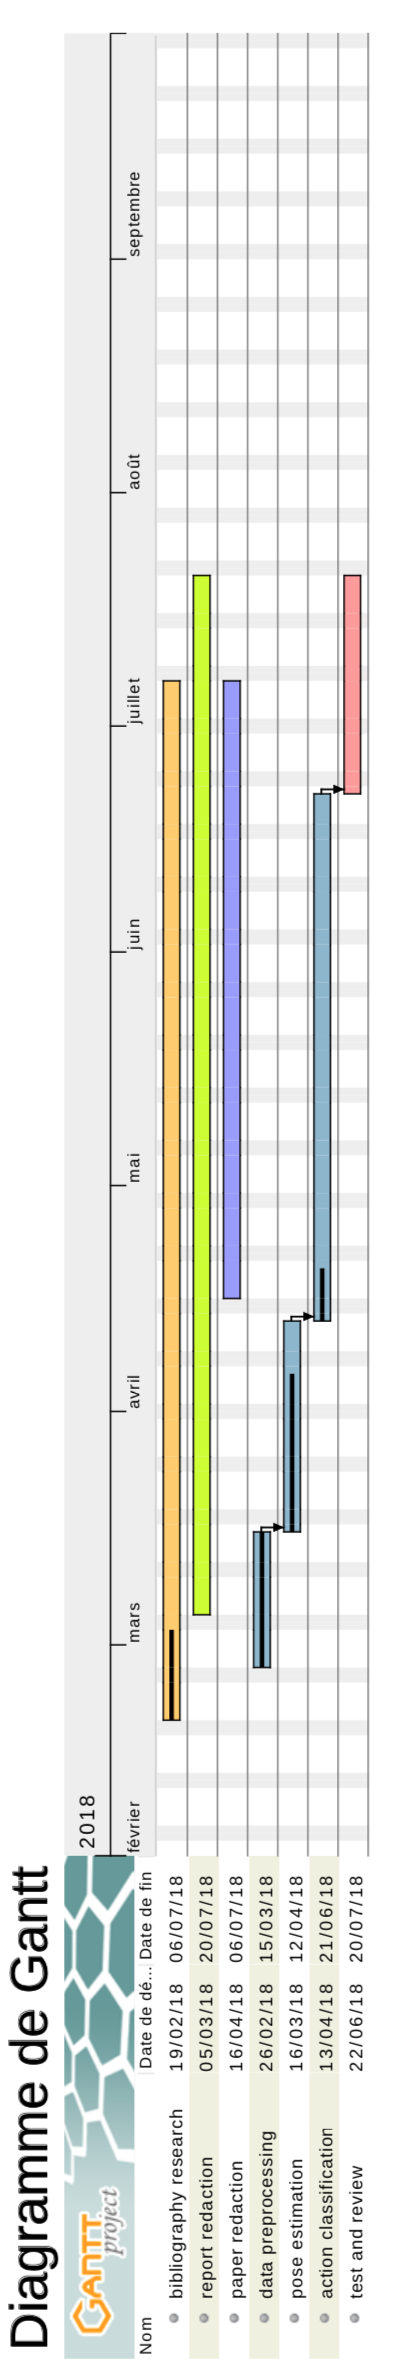
\includegraphics[width=0.2\textwidth]{images/gantt}
    \caption{Provisional schedule showing progress of the project}
\label{fig:gantt}
\end{figure}

\newpage

\section{Personal feedback}

\subsection{Work environment}
The first part of the internship consisted mainly of two tasks: bibliography search and data preprocessing. I started by looking for documentation regarding the state of the art of the divers steps of the project (pose estimation, action recognition, and pedestrian models). I find this part of the work extremely rewarding on the scientific level as it allows to discover new algorithms and methods. Even if most of the paper describe solutions that could not be applied on this specific project, I enjoyed reading them.

On a typical day of work, I arrive at the laboratory at 9:30AM and leave around 17:30PM (working 7.5 hours/day). I am suppose to share the laboratory with another french student, a chinese student and 10 japanese students. The six first weeks of my internship coincided with the end of the school year in Japan, so the laboratory was never actually full and most of the times we were only 4 or 5 working. Dr Akito Monden office is located in the same floor as the students office and Dr Yücel's office is located two floors lower. 

The overall ambience in the laboratory is great and the integration process went very smoothly, probably mainly because we are all students and because of the Japanese helpfulness and kindness. The furniture in the office also reflect this friendly environments, with bookshelves full of manga, coding books and retro console and games. A microwave and a fridge are also available directly in the office room. Once a week we all meet with the professors to eat together.

The project is publicly available on GitHub at \url{https://github.com/Chevrefeuille/walking-gesture-detection}. In a concern of privacy protection and size management, the videos are not available.

\subsection{Difficulties}
I relation to the project, the main difficulties that I experienced where linked with environment issues. I started working on my personal Mac Book Pro but many algorithms that I needed to use to test feasibility of considered solutions required an NVidia GPU. Indeed, most machine learning require heavy computation that is generally accelerated on GPU, very often using the CUDA toolkit that integrates well with traditional machine learning libraries such as Torch or Tensorflow. I started preprocessing the video data until I could use the wanted algorithms on a new computer.

\newpage

\section{Societal and environmental impact}

\subsection{Societal impact}
Considering the broader applications of pedestrian modeling, the possibilities in the field of robotic have in mind to help developing solutions to help smoothen interaction between automaton and human in the context of pedestrian movements. This could be used in a variety of way, such as guide or assistantship for disabled and elderly. 

The privacy aspect of the work can be discussed. Indeed, the videos show thousand of pedestrians that can easily be recognized given the quality of the clips. In a matter of privacy, all images shown in this report have the face blurred. Moreover, the dataset is not available in the public GitHub repository of the project.


\subsection{Environmental impact}
Regarding the environment, the first part of the project was fulfilled on my personal laptop computer. It was mainly used in battery mode, being charged around two hours per day. According to its technical documentation, this represents a power consumption of approximately 300Wh/day. For the 21 weeks of the internship, this correspond to a total consumption of around 30kWh.
The project will likely only take place in Okayama University laboratories. Except from the round trip from France to Japan, no further travels will be performed. Yet, this represents a substantial carbon footprint of 4t of CO2, almost twice the maximum amount that individuals should not exceed to prevent global warming. In terms of power consumption, this journey corresponds to more than 8000kWh, which is roughly equivalent to using 250 laptops during the duration of the internship. 

Moreover, Okayama being a very flat city, many people (and especially students) use bikes to move around. Likewise, I am using a bike to go to work therefore limiting my environmental impact. 

Japan is very involved in environmental procedure such as sorting of waste. In the laboratory office, we have two thrash can, one for the plastic bottles and another one for the rest of the trash. In the main buildings of the university, they are around 7 different trashes for various kind of waste: burnable, non burnable, cans, etc. 

\bibliography{pfe}{}
\bibliographystyle{plain}

\newpage

\appendix
\section{Contact information}


\begin{tabular}{@{}llll@{}} \toprule
    Name & Role & Email & Phone number \\ \midrule
    Adrien Gregorj & Intern & adrien.gregorj@gmail.com & +81 80 4099 5120 \\
    Dr Akito Monden & Supervisor &  monden@okayama-u.ac.jp & +81 86 251 8180 \\
    Dr Zeynep Yücel & Project supervisor & zeynep@okayama-u.ac.jp & +81 86 251 8245 \\
    Dr James L. Crowley & Ensimag supervisor & james.crowley@inria.fr & +33 4 76 61 53 96 \\ \bottomrule
\end{tabular}

\end{document}
